\subsection{추가 실험과 절제 분석}
\label{sec:ablations}

\subsubsection{Low-Rank Adaptation의 효과}

\label{sec:emb_lora_results}
\begin{table}[t]
\centering
\begin{tabular}{ll cr cr cr}
 & & \multicolumn{2}{c}{\textbf{PRAGMA-S}} & \multicolumn{2}{c}{\textbf{PRAGMA-M}} & \multicolumn{2}{c}{\textbf{PRAGMA-L}} \\
\cmidrule(lr){3-4} \cmidrule(lr){5-6} \cmidrule(lr){7-8}
\textbf{과제} & \textbf{지표} & \textbf{Emb.} & \textbf{LoRA} & \textbf{Emb.} & \textbf{LoRA} & \textbf{Emb.} & \textbf{LoRA} \\
\midrule
상품 추천 & mAP     & -- & +57.2\,\% & -- &  +68.4\,\% & -- &  +68.1\,\%    \\
\addlinespace
외부 사기        & Precision & -- &+30.8\,\% & -- & +29.8\,\% & -- & +23.8\,\% \\
                      & Recall    & -- & +27.4\,\% & -- & +24.5\,\% & -- & +13.3\,\% \\
\addlinespace
커뮤니케이션 인게이지먼트  & PR-AUC  & -- & +72.9\,\% & -- & +49.7\,\% & -- & +54.1\,\% \\
                          & ROC-AUC & -- & +16.9\,\% & -- & +11.2\,\% & -- & +13.5\,\% \\
\addlinespace
신용 평가        & PR-AUC     & -- & +18.0\,\% & -- & +20.4\,\% & -- &  +10.3\,\% \\
                      & ROC-AUC    & -- &  +0.2\,\% & -- &  +2.4\,\% & -- &  +1.5\,\% \\
\addlinespace
정기 거래 & $F_\text{1}$ & -- & +4.5\,\% & -- &  +3.2\,\% & -- &  +2.3\,\% \\
\addlinespace
라이프타임 밸류        & PR-AUC     & -- & +3.6\,\% & -- &  +2.4\,\% & -- &  +2.9\,\% \\
                      & ROC-AUC    & -- & +4.7\,\% & -- &  +3.4\,\% & -- &  +3.9\,\% \\
\end{tabular}
\caption{\textbf{스케일별로 본 LoRA 튜닝 모델의 임베딩 전용 베이스라인 대비 상대 향상.}
각 모델 크기(S, M, L)에서 임베딩 전용 변형을 기준(Emb)으로 사용한다.
성능 이득은 ($\text{LoRA} / \text{Emb} - 1$)로 계산한다.}
\label{tab:lora_vs_emb_scaling}
\end{table}

표~\ref{tab:lora_vs_emb_scaling}이 보여 주듯, 평가된 모든 과제와 모델 스케일에서 LoRA 튜닝 변형은 임베딩 전용 베이스라인을 일관되게 능가한다. 이는 고정 임베딩이 놓칠 수 있는 과제별 미묘한 신호를 파라미터 효율적 파인튜닝이 잘 포착함을 보여준다.
가장 두드러진 향상은 커뮤니케이션 인게이지먼트에서 관찰되며, Small 모델에서 LoRA가 PR-AUC를 +72.9\,\% 끌어올리고, Medium·Large 변형에서도 큰 차이를 유지한다.
신용 평가에서는 Medium 모델의 PR-AUC가 +20.4\,\%로 가장 큰 상대 향상을 기록한다. 이는 복잡한 분류 과제에서 그 스케일의 LoRA 레이어가 특히 효과적임을 시사한다.
정기 거래와 LTV의 이득은 더 작아, 보통 +2.3\,\%에서 +4.7\,\% 범위에 있다.


\subsubsection{프로필 상태의 효과}
\label{sec:effect_profile_state}

표~\ref{tab:pragma_s_results}는, 전체 PRAGMA-S 모델과 프로필 상태 가지(branch)를 완전히 제거하고 이벤트 수준 표현에만 의존하는 변형을 비교함으로써 프로필 상태 인코더~(\S\ref{sec:architecture})의 기여를 분리해 보여 준다.
영향은 과제에 따라 강하게 달라진다.
신용 평가는 큰 이득을 본다 — PR-AUC에서 +31.8\,\%, ROC-AUC에서 +4.9\,\%의 상대 이득.
PR-AUC가 유난히 크게 오른 것은, 계정 보유 기간이나 온보딩 특성 같은 정적 신호가 소수 클래스인 채무 불이행을 식별하는 데 특히 유용한 변별적 맥락을 제공한다는 것을 의미한다 — 이는 이벤트 시퀀스만으로는 충분히 잡아내기 어렵다.
대조적으로, 라이프타임 밸류에서는 PR-AUC +2.2\,\%, ROC-AUC +2.0\,\%로 이득이 더 적어, 매출총이익 가능성은 예측 지평에 걸친 거래 패턴만으로도 상당 부분 추론 가능함을 시사한다.
커뮤니케이션 인게이지먼트는 PR-AUC가 살짝 회귀($-$3.0\,\%)하면서 ROC-AUC는 미미하게 상승(+1.3\,\%)한다. 이는 재인게이지먼트 성향이 정적 사용자 특성보다는 이탈 직전 이벤트 패턴에 거의 전적으로 좌우됨을 가리킨다.
이 결과들은 PRAGMA의 두 가지 가지(branch) 설계를 검증한다 — 정적 프로필 상태가 정보적인 과제에서는 전용 프로필 상태 인코더가 의미 있는 가치를 더해 주고, 그 신호가 덜 관련된 과제에서는 아키텍처가 우아하게 성능을 유지한다.

\begin{table}[t]
\centering
\begin{tabular}{llcr}
& & \multicolumn{2}{c}{\textbf{PRAGMA-S}} \\
\cmidrule(lr){3-4}
\textbf{과제} & \textbf{지표} & \textbf{Event-only (기준)} & \textbf{Full} \\
\midrule
외부 사기           & Precision  & -- & +46.8\,\% \\
                         & Recall     & -- & +85.6\,\% \\
\addlinespace
신용 평가           & PR-AUC     & -- & +31.8\,\% \\
                         & ROC-AUC    & -- & +4.9\,\% \\
\addlinespace
상품 추천   & mAP        & -- & +3.5\,\% \\
\addlinespace
라이프타임 밸류           & PR-AUC     & -- & +2.2\,\% \\
                         & ROC-AUC    & -- & +2.0\,\% \\
\addlinespace
정기 거래   & $F_\text{1}$ & -- & +2.4\,\% \\
\addlinespace
커뮤니케이션 인게이지먼트 & PR-AUC     & -- & $-$3.0\,\% \\
                         & ROC-AUC    & -- & +1.3\,\% \\
\end{tabular}
\caption{
    \textbf{프로필 상태는 정적 사용자 특성이 변별적인 과제에 큰 기여를 한다.}
    상대 성능은 ($\text{Full} / \text{Event-only} - 1$)로 계산한다.
}
\label{tab:pragma_s_results}
\end{table}

\subsubsection{커뮤니케이션 인게이지먼트(Uplift)}
\label{sec:credit_engagement_communications_uplift}

이 과제는 단순한 전환 예측을 넘어, 중단된 신용 신청 사용자를 다시 끌어들이는 데 어떤 메시징 전략이 가장 효과적인지를 식별하는 \emph{최적 처치 선택}으로 나아간다.
데이터셋은 다른 다운스트림 벤치마크보다 작지만, 이 과제에서는 대규모 사전학습이 결정적인 역할을 한다 — 제한된 인-도메인 데이터만으로 학습된 베이스라인을 큰 폭으로 능가한다.
업리프트(uplift) 과제이기에 평가의 각도도 다르다 — PRAGMA는 파인튜닝되지 않고 동결된 피처 추출기로 사용되어 메타러너에 입력되며, 따라서 과제별 적응 없이 표현 자체의 품질을 분리해 평가할 수 있다.

구체적으로, 저자들은 이질적 처치 효과(heterogeneous treatment effects)를 추정하는 메타러너 프레임워크~\citep{kunzel2019metalearners}를 채택하며, 모델이 이탈 직전 이벤트 신호, 프로필 상태, 처치 할당 사이의 복잡한 상호작용을 포착하도록 요구한다.
PRAGMA와 베이스라인 모두 동일한 메타러너를 사용하며, 차이는 그 안의 표현(representation)뿐이다.

표~\ref{tab:uplift_results}는 Area Under the Uplift Curve(AUUC)와 SNIPS~\citep{swaminathan2015self}를 사용한 결과를 정리한다.
잠재된 이벤트 수준 패턴을 포착하는 PRAGMA-L의 능력은 매우 효과적인 처치 할당으로 이어져, 내부 베이스라인 대비 AUUC를 163.7\,\% 상대 증가시킨다.

\begin{table}[t]
\centering
\begin{tabular}{llcr}
\textbf{과제}               & \textbf{지표}   & \textbf{베이스라인 (기준)} & \textbf{PRAGMA} \\
\midrule
커뮤니케이션 인게이지먼트 (uplift) & AUUC       & --                     & +163.7\,\%                \\
                           & SNIPS             & --                     &  +10.8\,\%                \\
\end{tabular}
\caption{
    \textbf{동일한 메타러너 프레임워크에서 PRAGMA-L과 내부 업리프트 베이스라인의 성능 비교.}
    상대 성능은 ($\text{PRAGMA-L} / \text{Baseline} - 1$)로 계산한다.
    }
    \label{tab:uplift_results}
\end{table}

\subsubsection{사전학습된 텍스트 인코더의 효과}
\label{sec:external_embeddings}

표준 PRAGMA 아키텍처에서는 텍스트 값이 다른 모든 표 형식 피처와 함께 임베딩 룩업 테이블을 통해 공동 학습된다(\S\ref{sec:token_embedding} 참조).
모델이 희소하거나 잡음이 많거나 매우 불규칙한 금융 텍스트(예: 잘린 거래 설명)에 과소적합되지 않도록, 저자들은 텍스트 이해를 별도의 사전학습된 텍스트 임베딩 모델(예: Nemotron-1B-v2~\citep{moreira2024nvretriever})로 분리하는 안을 검토한다.
이 분리된(decoupled) 접근은 더 풍부한 즉시 사용 의미 표현을 제공하면서, 주된 이벤트 트랜스포머~(\S\ref{sec:event_encoder})가 피처 간 상호작용에 집중할 수 있게 해 준다.
이 변형을 일반화된 코어 아키텍처의 기본으로 채택하지는 않지만, 도메인 특화 통찰을 주는 선택적 확장으로 보고한다.

\paragraph*{구현 세부.}
사전학습된 텍스트 인코더의 추가는 PRAGMA 아키텍처에 여러 구조적 변경을 동반한다.
첫째, 보통 자체 학습된 BPE 토크나이저와 학습 가능한 임베딩 룩업 테이블로 인코딩되던 의미 타입(키)들의 값에 대해, 대신 동결된 사전학습 모델로 전체 텍스트 문자열을 단일 벡터로 매핑한 뒤, 한 층(one-layer)의 학습 가능한 사영을 통해 적응시킨다(그림~\ref{fig:external_emb_arch} 참조).
둘째, MLM 최적화(\S\ref{sec:training} 참조) 동안 이 텍스트 필드의 정확한 토큰 라벨을 복원하는 대신, 사전학습된 텍스트 인코더가 만들어 내는 연속(continuous) 텍스트 임베딩을 평균제곱오차(MSE)로 복원하도록 PRAGMA를 학습시킨다.


\begin{figure}[t]
    \centering
    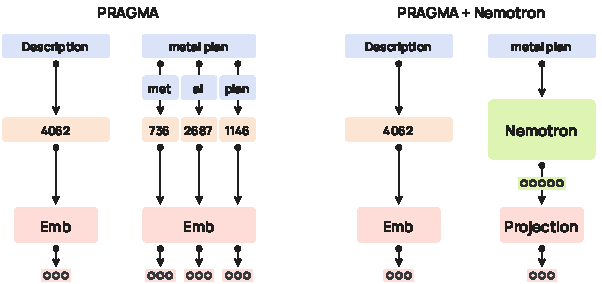
\includegraphics[width=0.7\linewidth]{images/pt_text_embs.pdf}
    \caption{
        \textbf{PRAGMA의 텍스트 임베딩(왼쪽)과 사전학습 Nemotron-1B-v2 텍스트 임베딩 사용 버전(오른쪽) 비교}.
        자체 학습 BPE 토크나이저와 학습 가능한 임베딩 룩업 테이블 대신, 사전학습된 ``동결'' Nemotron이 텍스트 값 전체를 단일 텍스트 임베딩 벡터로 매핑하고, 학습 가능한 사영으로 트랜스포머의 기본 차원에 투영한다.
    }
    \label{fig:external_emb_arch}
\end{figure}

\paragraph*{결과 및 논의.}
결과는 표~\ref{tab:pretrained_text_embedding}에 제시한다.
다운스트림 효과는, 자유 텍스트와 범주형·행동 구조 가운데 어느 쪽에 라벨 관련 신호가 더 많이 들어 있는지에 따라 갈린다.
신용 평가는 가장 명확한 상승을 보인다 — Nemotron 사용 시 PR-AUC가 상대 +16.1\,\%, ROC-AUC가 +2.8\,\% 향상된다.
반면 상품 추천은 손실을 본다 — mAP가 상대 6.4\,\% 떨어지는데, 이는 희소한 텍스트가 구조적 채널이 이미 인코딩하고 있는 정보 위에 별 추가 정보를 주지 않기 때문으로 보인다.
외부 사기는 정밀도(+3.8\,\%)와 재현율($-$0.7\,\%)에서 작은 폭으로 반대 방향으로 움직이고, LTV와 정기 거래는 보고된 지표상 거의 변동이 없다.
이 변형은 또한 PRAGMA-M 학습 지연을 약 18\,\% 늘리기 때문에, 저자들은 이를 기본 아키텍처에 포함시키는 대신 텍스트 비중이 큰 과제에서 옵트인하는 모듈로 유지한다.

\begin{table}[t]
\centering
\begin{tabular}{llcr}
& & \multicolumn{2}{c}{\textbf{PRAGMA-M}} \\
\cmidrule(lr){3-4}
\textbf{과제}            & \textbf{지표} & \textbf{기준} & \textbf{+Nemotron} \\
\midrule
신용 평가           & PR-AUC          & --                     & +16.1\,\%                   \\
                         & ROC-AUC         & --                     &  +2.8\,\%                   \\
\addlinespace
정기 거래   & $F_\text{1}$    & --                     &  +0.1\,\%                   \\
\addlinespace
라이프타임 밸류           & PR-AUC          & --                     &  +0.8\,\%                   \\
                         & ROC-AUC         & --                     &  +0.6\,\%                   \\
\addlinespace
외부 사기           & Precision       & --                     &  +3.8\,\%                   \\
                         & Recall          & --                     &  $-$0.7\,\%                   \\
\addlinespace
상품 추천   & mAP             & --                     &  $-$6.4\,\%                  \\
\end{tabular}
\caption{
    \textbf{사전학습된 텍스트 임베딩의 다운스트림 영향은 텍스트 비중이 큰 도메인에 집중된다.}
    성능은 LoRA 튜닝된 PRAGMA-M 대비 추정한 값이다.
}
\label{tab:pretrained_text_embedding}
\end{table}

\subsubsection{높은 관계성을 가진 과제의 한계: 자금세탁방지(AML)}
\label{sec:aml}
저자들은 자금세탁방지(Anti-Money Laundering, AML)를 이진 분류 과제로 정식화한다.
표~\ref{tab:aml_results}에서 보이듯, 이 과제는 PRAGMA가 운영 베이스라인보다 크게 뒤지는 설정이다.

저자들은 이 성능 격차를 두 가지 주된 요인으로 본다.
첫째, AML 다운스트림 데이터셋은 베이스라인 모델이 파운데이션 수준의 사전학습 없이도 견고한 과제별 표현을 학습하기에 충분히 크다.
둘째, 그리고 더 결정적으로, AML 탐지는 본질적으로 \emph{관계적(relational)} 이다 — 베이스라인은 네트워크 수준 신호를 포착하는 레코드 간(cross-record) 피처를 활용한다.
PRAGMA는 이벤트 이력을 고립된 단위로 처리하므로, 만들어진 임베딩은 이 과제에 결정적인 레코드 간 의존 구조를 본질적으로 담지 못한다.

성능은 정밀도를 강조하면서도 재현율을 함께 반영하는 $F_\text{0.5}$를 주된 지표로 평가한다.
PRAGMA는 네트워크-인지 베이스라인 대비 $F_\text{0.5}$가 47.1\,\% 떨어지며, 이는 고립된 레코드 수준 표현이 이 강한 관계성 도메인에서는 충분하지 않을 수 있음을 보여준다.
이 한계를 해소하는 것은 향후 연구의 핵심 방향이다.

\begin{table}[t]
\centering
\begin{tabular}{llcr}
\textbf{과제}               & \textbf{지표}   & \textbf{베이스라인 (기준)} & \textbf{PRAGMA} \\
\midrule
자금세탁방지(AML)       & $F_\text{0.5}$    & --                     & $-$47.1\,\%        \\
\end{tabular}
\caption{
    \textbf{자금세탁방지 과제에서 PRAGMA와 베이스라인의 성능 비교.}
    상대 성능은 PRAGMA-L 임베딩 위 선형 프로브로 ($\text{PRAGMA} / \text{Baseline} - 1$)으로 계산한다.
    }
    \label{tab:aml_results}
\end{table}
